%!TEX root = Nanomat.tex
\ctitle{Katalyse med metall-nanopartikler}
\paragraph{Poenget med metall-nanopartikler} Metall-nanopartikler er særlig brukt til katalyse, og lages ofte av kostbare metaller som palladium, sølv, platina eller gull. Siden katalyse (i likhet med alle andre kjemiske reaksjoner) skjer på overflaten av materialet, ønsker vi at katalysatorene skal bestå av så mye overflate som mulig\footnote{Så mye overflate som mulig, og så lite dybde som mulig. Akkurat som dette emnet! ZING!} - derfor vil vi ha metallene i form av nanopartikler.

\cstitle{Størrelseseffekter}
Størrelseseffekter refererer til endringene i metallets egenskaper når partiklene det består av er veldig små. Igjen: størrelseseffekter forårsakes av to ting:  \emph{økt andel atomer med lavt koordinasjonstall} \emph{endring i elektronstruktur/kvantemekaniske effekter}.

\paragraph{Økt andel atomer med lavt koordinasjonstall} Katalyse skjer, veldig forenklet, i to trinn:
\begin{enumerate}
	\item Reaktantene adsorberes på overflaten av katalysatoren, og bindingene i reaktantene brytes der.
	\item Reaktantene reagerer med hverandre og desorberes fra katalysatoren.
\end{enumerate}
Når katalysatorene er i form av bittesmå partikler, kan det medføre både fordeler og ulemper. Siden vi har mange reaktive atomer, er det lettere å få til trinn 1. Men det blir også vanskeligere å få til trinn 2. Hvis vi ikke får til trinn 2, vil katalysatoren raskt bli dekket med reaktant, og reaksjonen vil opphøre.

\paragraph{FCC-nanopartikler} FCC\footnote{Den riktige/vanlige måten å skrive forkortelser for krystallstrukturer på, er å bruke små bokstaver, altså ``fcc'' i stedet for ``FCC''. Personen som fant på denne konvensjonen lever ikke lenger, jfr. fotnote 15.}-strukturen er tettpakket, og i bulkmaterialet har hvert atom et koordinasjonstall på 12. Wullf-polyederet til FCC-strukturen er et avstumpet oktaeder, og det er slik FCC-partikler ser ut når de blir tilstrekkelig store.

Noen FCC-metaller, som kobber og sølv, foretrekker å danne et ikosaeder (som er en ikke-krystallin struktur) når partiklene består av færre enn ca. 100 atomer, mens palladium, platina og gull danner avstumpede oktaedere allerede ved et noen titalls atomer.

En ting som kan være viktig å få med seg om FCC-nanopartikler er at overflateatomer med samme koordinasjonstall ikke nødvendigvis har samme elektroniske miljø:
\begin{itemize}
	\item overflateatomet som er nabo til en kant, har et annet miljø enn overflateatomet som er midt i en flate.
	\item et atom på en kant mellom to $(111)$-plan har et forskjellig elektronisk miljø fra et atom på en kant mellom et $(100)$-plan og et $(111)$-plan.
\end{itemize}

\paragraph{Effekter ved overflaten} Ved overflaten skjer det flere spennende ting:
\begin{itemize}
	\item Avstanden mellom to atomer på overflaten er mindre enn avstanden mellom to atomer i bulk.\footnote{Man kan kanskje se på det som at atomene prøver å gjøre opp for de tapte bindingene sine ved å binde seg sterkere til atomene som er igjen.} 
	\item Atomene på overflatene trekker seg også sammen med atomene rett under seg. Jo lavere koordinasjonstall atomet på overflaten har, jo mer trekker det seg inn mot atomene under seg. Dette har blitt vist i nikkel: på det tettpakkede $(111)$-planet er avstanden mellom ytterste og nest ytterste atom 1-2\% mindre enn gitterparameteren. På det mindre tettpakkede $(111)$-planet er denne sammentrekningen nærmere 10\%.
	\item Hvis det adsorberes reaktanter på overflaten av nanopartiklene, vil det ikke lenger være løse bindinger der. Derfor vil adsorberte reaktanter forminske de ovennevnte effektene.
\end{itemize}

\paragraph{Endring i smeltepunkt, Lindemannkriteriet} Lindemannkriteriet er en definisjon av smelting: at man regner et (bulk)material som smeltet når de interatomære avstandene fluktuerer med mer enn 10\% av gitterparameteren. Siden atomer på overflaten er friere til å bevege seg enn de i bulk, vil en større andel overflateatomer føre til at dette kriteriet oppnås ved en lavere temperatur enn i bulkmaterialet. Dermed er smeltepunktet lavere for små partikler.

Et eksempel på konsekvensene av dette er produksjon av karbonnanorør med \ce{Ni}-nanopartikler som katalysator. Hvis man kjører denne prosessen ved \SI{800}{\celsius} får man en ganske annen morfologi enn hvis man gjør det ved \SI{700}{\celsius}. Forklaringen på dette er at smeltepunktet for de katalyserende nanopartiklene er et sted mellom disse temperaturene.

\cstitle{Endringer i elektronisk struktur}
For bulkmaterialer brukes \emph{valensbånd} og \emph{ledningsbånd} for å skille mellom metaller, halvledere og isolatorer. Forutsetningen for å kunne bruke en slik modell, er at man har et tilnærmet uendelig antall atomer, og at disse påvirker hverandres elektronstruktur. Den samlede effekten av alle disse gjensidige elektroniske påvirkningene er at det oppstår utallige forskjellige energinivåer som hvert enkelt elektron i materialet kan ``velge mellom''. Vi vet fra kvantemekanikken at det \emph{egentlig} bare finnes et endelig antall energinivåer for hvert elektron, men når materialet består av mange atomer, er tilnærmingen god. 

Tilnærmingen krever modifisering når nanopartiklene består av et antall partikler som ikke kan tilnærmes med uendelig. For det første: når partiklene blir små, minker bredden på energibåndene, og det begynner å oppstå energigap. Etter hvert blir de så tynne at materialer som i bulkform er metaller, blir til halvledere og til slutt elektriske isolatorer.  For det andre: når partiklene består av et ett- eller tosifret antall atomer, endres de elektroniske egenskapene plutselig og uforutsigbart avhengig av størrelse (se figur 10.5 i Bréchnigac). For å beskrive de elektroniske egenskapene til så små partikler, kreves en ordentlig kvantemekanisk analyse.

Et eksempel på ``bruk'' av størrelsesavhengig elektronisk struktur er fotoluminescens i \ce{CdSe}-nanopartikler med diameter på mindre enn \SI{10}{\nano\meter}. Slike partikler er halvledende, og har et energigap $E_g$ som avhenger av størrelsen på partikkelen. Hvis man lyser på partiklene, lyser partiklene tilbake med en viss farge. Fargen avhenger av $E_g$ og dermed altså av størrelsen på partiklene. Check it out:
\begin{figure}[H]
	\centering
	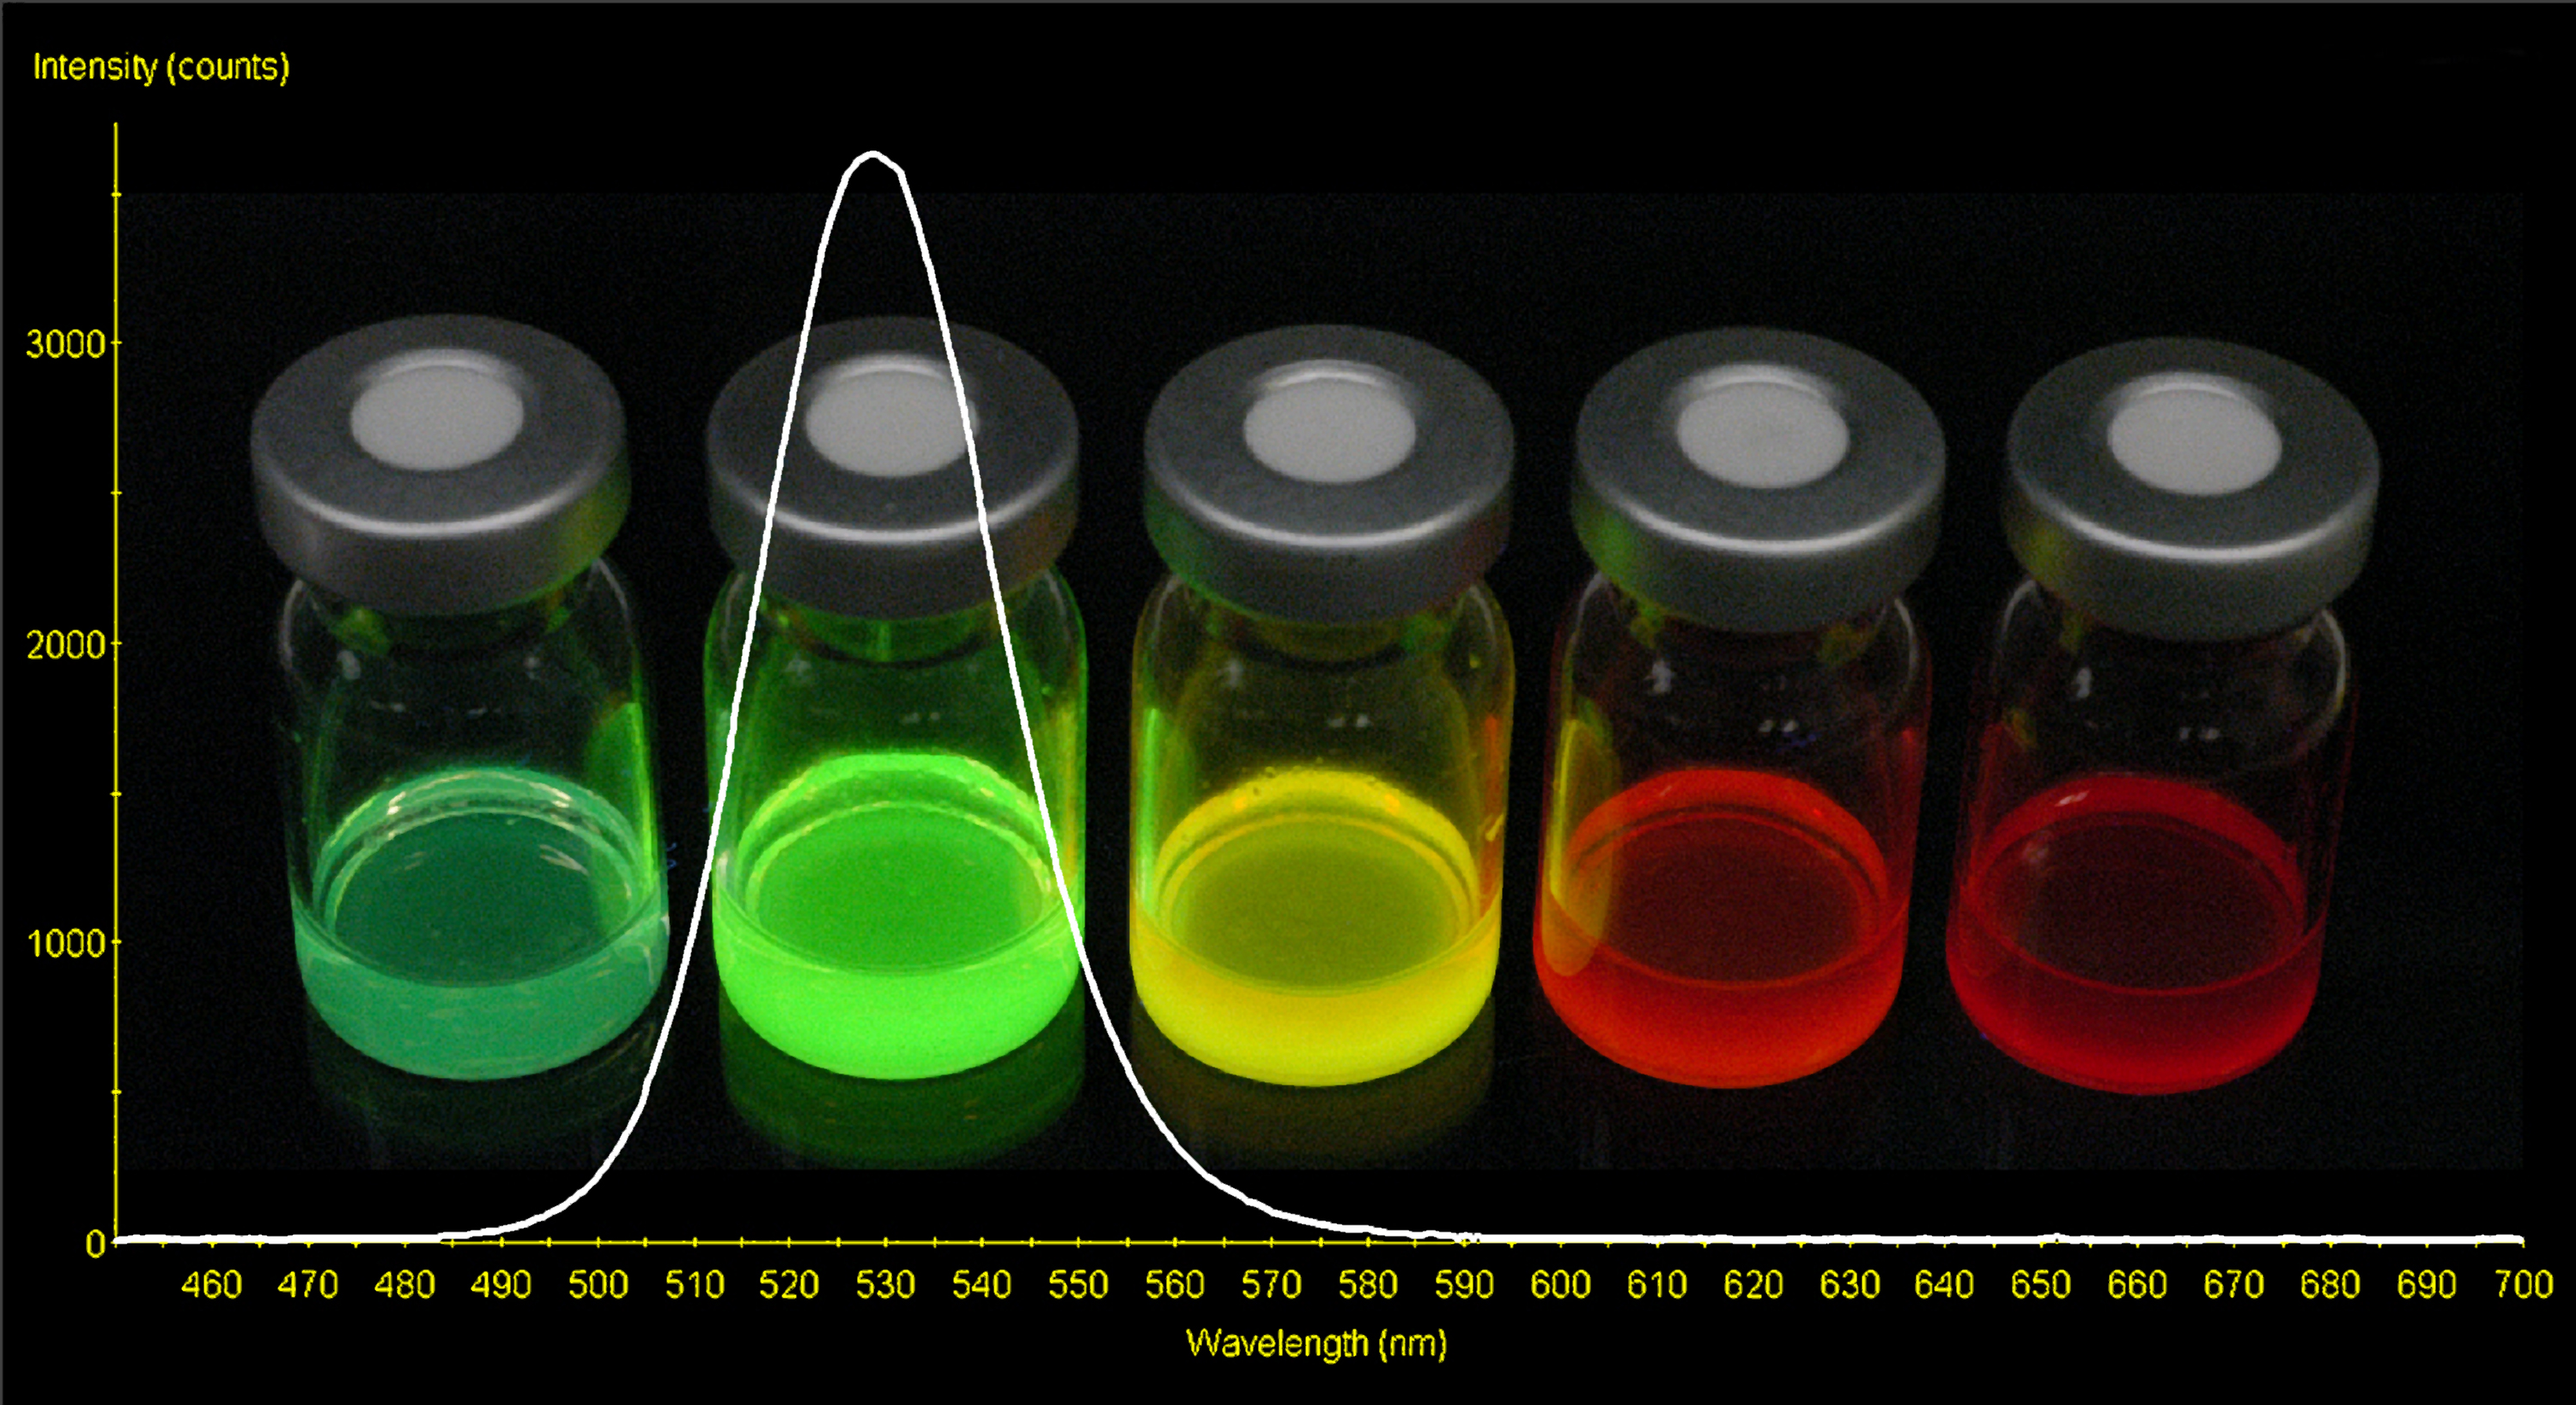
\includegraphics[width=0.95\linewidth]{CdSeqdots.jpg}
	\caption{\ce{CdSe}-kvanteprikker, av forskjellig størrelse, som har blitt bestrålt med UV-lys. Og en graf. Jeg tror grafen beskriver strålingen fra den grønne løsningen.}
	\label{fig:qdots}
\end{figure}

\cstitle{Legeringseffekter}
Egenskapene til katalysatoren kan endres når man legger til et annet metall. En legering av to metaller kan være en bedre katalysator enn begge metallene er hver for seg. Dette har å gjøre med ting som at det aktive setet på en katalysator består av mer enn ett atom, og at legeringer er komplekse greier.

\paragraph{Overflatesegregering} Det er gjerne slik at de atomene som har lavest overflatespenning beveger seg ut mot overflaten, for å minimere overflateenergien til partikkelen som helhet. Det vil særlig være større andel atomer med lav overflatespenning på fasettene som har lavt koordinasjonstall, og på kanter og hjørner. Hvis atomet attpåtil har stor atomradius, blir effekten enda sterkere.

Her er et eksempel på når det kan være nyttig. Man kan lage hydrogen i reaksjonen \ce{2H2O + CH4 -> CO2 + 4H2}, katalysert med \ce{Ni}. Men da pleier karbon å feste seg til nikkelatomene på kanter/hjørner og ikke gi slipp, slik at katalysatoren blir deaktivert og reaksjonen stopper etter kort tid. For å løse dette legger vi til litt \ce{Au}, for gull har lavere overflatespenning enn nikkel, og gullatomene vil bevege seg mot kantene og hjørnene. Karbonet binder seg ikke like bra til gull, så vi får en \emph{bedre katalysator} selv om vi har lagt til noen \emph{mindre reaktive} gullatomer.

Overflatesegregering kan begrenses dersom atomer av forskjellig type binder seg sterkere til hverandre, enn hver type atomer binder seg til hverandre hver for seg --- altså dersom
\begin{equation}
	\Delta H_{\ce{A-B}} > \frac{1}{2}\left(\Delta H_{\ce{A-A}} + \Delta H_{\ce{B-B}}\right).
\end{equation}
Effekten begrenses naturligvis også av at termisk energi mikser og trikser med atomene, ellers ville den minste forskjell i overflatespenning forårsaket fullstendig segregering for legeringer der ulikheten over ikke holder.

\paragraph{Fortynningseffekt} Noen katalytiske reaksjoner krever at man har en sammenhengende gruppe med flere atomer av samme type. Hvis overflaten fortynnes med andre atomer, vil det finnes færre slike steder, så disse reaksjonene vil skje sjeldnere. Andre reaksjoner, som \emph{ikke} krever en slik sammenhengende gruppe, vil ikke påvirkes i samme grad. Hvis det vi ønsker oss er reaksjoner av den sistnevnte typen, bør vi bruke en legering for å øke selektiviteten til katalysen.

\paragraph{Effekter på elektronisk struktur} Interaksjoner mellom de to metallene kan endre elektronstruktur gjennom ting som kjemisk binding, ladningsoverføring, polarisering og spenninger i krystallgitteret. Dette vil igjen påvirke reaktiviteten til det katalyserende metallet. Det er ofte vanskelig å finne ut hva som forårsaker hva.
